\section{The Clinical Control Problem}
\label{sec:clinical-problem}

Identifying an optimal seizure-management strategy requires more than describing which patients do
well. It requires representing seizure treatment as what it is in practice: a dynamic control
problem, in which clinicians repeatedly observe electrographic disease burden and adjust
anti-seizure medication in response, so that treatment and disease evolution shape one another over
time. This section states the problem and fixes the notation used for the rest of the paper. It
deliberately stops short of any result; the framework is developed in Sections~\ref{sec:prelim}--\ref{sec:estimation}
and evaluated in Section~\ref{sec:results}.

\subsection{Notation}
\label{sec:notation}

We observe patients at discrete times $t \in \{0,1,2,\ldots\}$ over a 168-hour horizon, and write
$\bar{Z}_t$ for the history of a variable $Z$ through time $t$.

\begin{itemize}\setlength{\itemsep}{2pt}
\item $L_t$ --- \textbf{epileptiform-activity burden}, a scalar summary of EEG severity at time $t$.
This is the quantity clinicians titrate against, and the input to the feedback controller defined
below. Section~\ref{sec:eeg-readout} discusses what is lost in reducing an EEG to a scalar, and what
a real deployment would require of this measurement.

\item $L_{0,t}$ --- the \textbf{natural history}: the burden that would have been observed at time
$t$ under no treatment. $L_t$ and $L_{0,t}$ coincide in untreated patients and diverge under
therapy.

\item $X$ --- baseline clinical covariates (age, SOFA score).

\item $A_t$ --- treatment intensity at time $t$; a continuous, non-negative infusion rate.

\item $\theta$ --- the \textbf{target epileptiform-activity threshold}: the level of $L_t$ that a
given treatment policy attempts to maintain. A policy is indexed by $\theta$; smaller $\theta$ means
more aggressive suppression.

\item $C_{t+1}$, $Y_{t+1}$ --- censoring and death indicators for the interval $(t,t+1]$.

\item $H_t = (X, \bar{L}_t, \bar{A}_{t-1})$ --- the \textbf{observed history} through time $t$:
baseline covariates together with all severity measurements and all treatment decisions made up to
that point. This is the conditioning set on which the identification assumptions of
Section~\ref{sec:prelim} are stated.
\end{itemize}

The distinction between $L_t$ and $H_t$ is used throughout and is worth stating once explicitly. A
treatment policy is a rule for setting $A_t$ from the current scalar severity $L_t$---that is what a
clinician titrating at the bedside actually does. Valid causal identification, by contrast, requires
conditioning on the entire history $H_t$, including baseline covariates and past treatment. The two
objects serve different purposes: $L_t$ defines \emph{what the policy is}, and $H_t$ defines
\emph{what must be adjusted for} in order to estimate the policy's effect.

\subsection{Variation in Clinical Practice}

Figure~\ref{fig:control-problem}A--C shows three treatment patterns commonly seen in ICU care. The
untreated patient (panel A) follows the natural history---a characteristic rise and fall that,
though eventually self-resolving, often proves fatal before resolution; this occurs when the
treating physician judges treatment more harmful than beneficial. The dose-changing patient (panel
B) receives intermittent adjustments. The closed-loop patient (panel C) is titrated continuously to
hold burden below a target ($\theta = 0.1$ in this illustration).

The intermittent adjustments in panel B are not meant to suggest arbitrary decision-making. They
reflect the episodic, coarse changes that arise from sedation interruptions for neurologic
examination, delayed response to evolving EEG findings, clinician hand-offs, and the absence of
automated titration. Collectively these patterns reflect the absence of consensus on treatment
strategy~\cite{chong2005which, rubinos2018ictal, osman2018ictal, johnson2017population, tao2020ictal, cormier2017ictal}---and
it is precisely this variation that makes observational learning possible, since a population in
which every patient were treated identically would carry no information about alternatives.

\subsection{Closed-Loop Feedback Control}

We take closed-loop control as the natural class of treatment strategies to study. Such a policy
adjusts medication to give no more and no less than needed to keep epileptiform activity below a
target level~\cite{astrom2010feedback, an2017design, westover2015robust, fialho2009closed};
Figure~\ref{fig:control-problem}D gives the schematic. The clinical team is modeled as a controller
that sets treatment intensity $A_t$ from the error $e_t = L_t - \theta$ between observed burden and
target. The patient's response is governed by their natural history $L_{0,t}$ and their individual
pharmacokinetic--pharmacodynamic (PKPD) profile. The result is a closed loop in which treatment and
disease activity are each a function of the other's history.

Two consequences follow, and they organize the rest of the paper. First, within this class,
\emph{asking what treatment is optimal reduces to asking what value of $\theta$ is optimal}---the
search over strategies becomes a search over a single interpretable parameter. Second, the same
feedback that makes the policy clinically sensible is what makes the data hard to analyze: because
$A_t$ depends on $L_t$, and $L_t$ depends on $\bar{A}_{t-1}$, disease severity is simultaneously a
confounder of later treatment and a mediator of earlier treatment. Conditioning on it introduces
bias; ignoring it introduces bias. This is the structure that the g-formula, introduced in
Section~\ref{sec:prelim}, is designed to handle, and that standard adjustment cannot.

\begin{figure}[htbp]
\centering
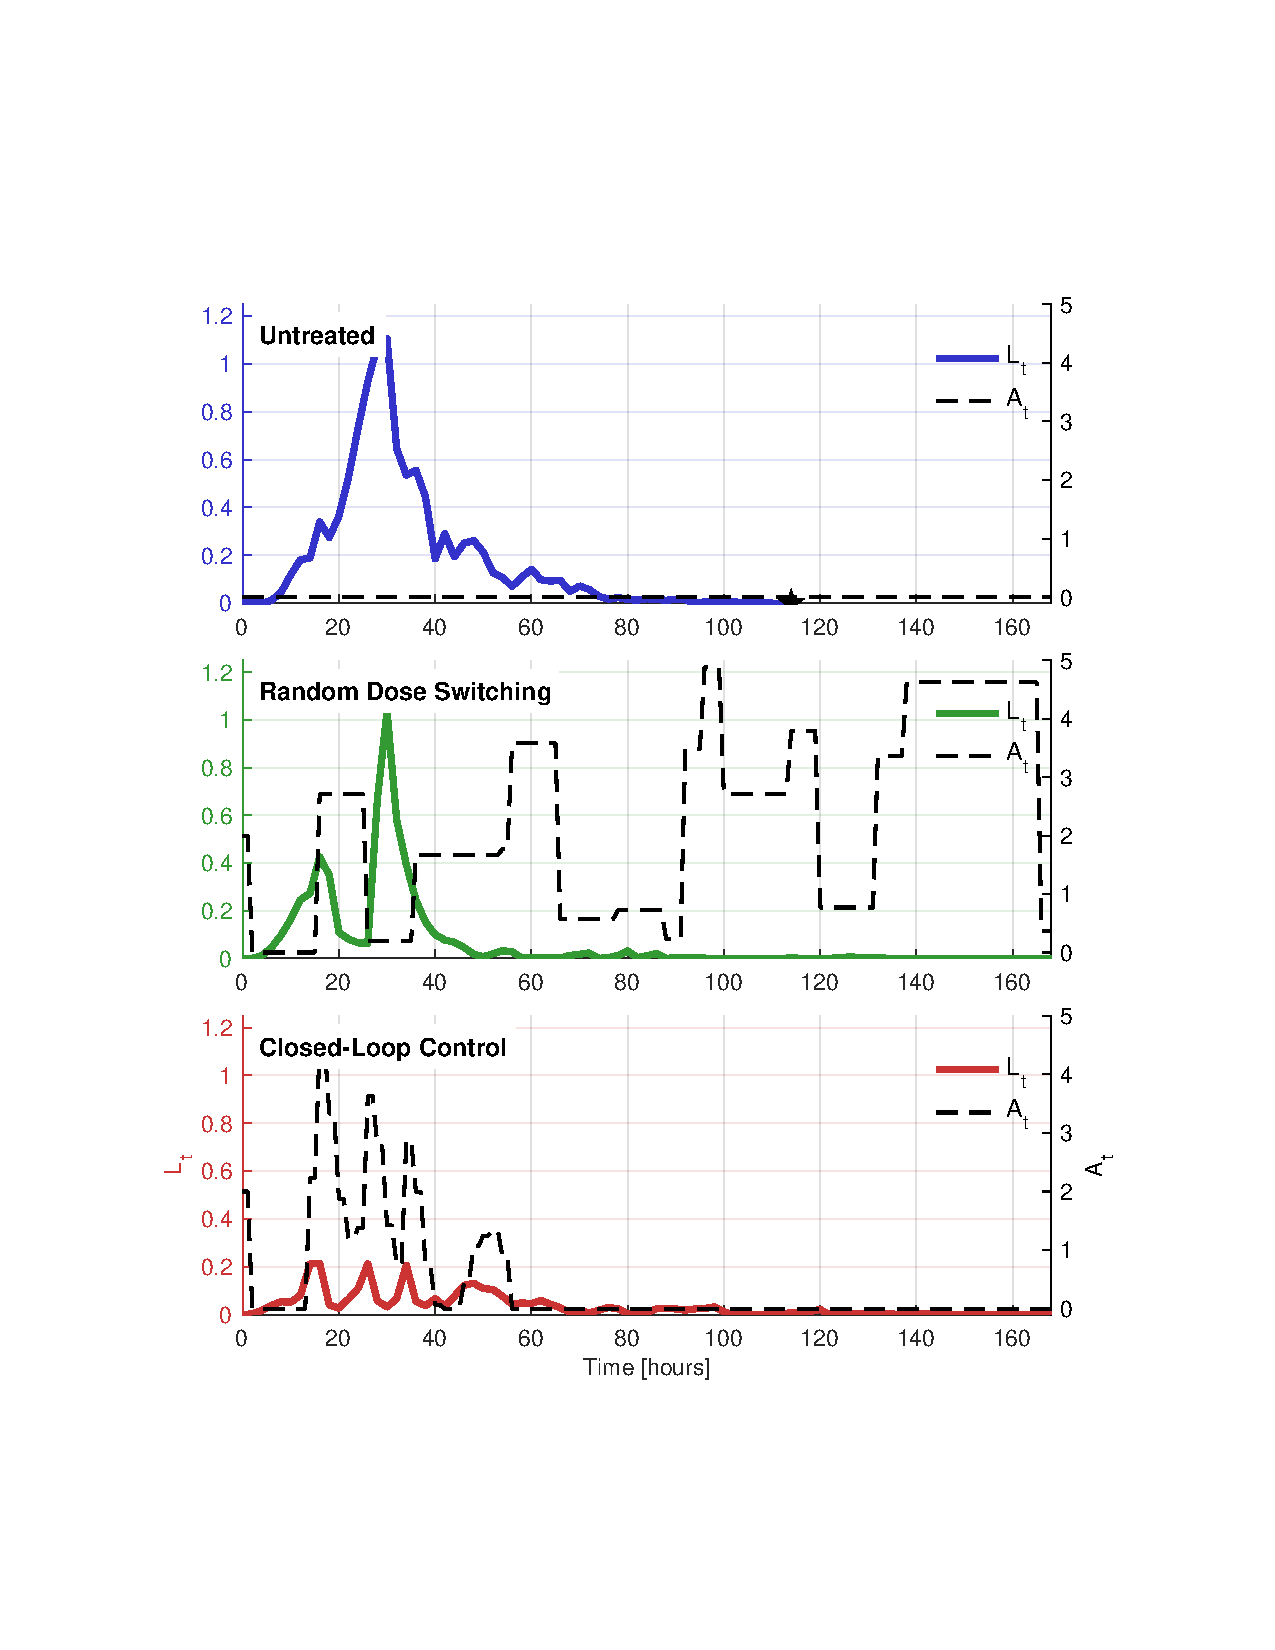
\includegraphics[width=\linewidth, trim=2.25cm 4.5cm 2.25cm 2cm, clip]{Fig1_singleTrajectories_3panels.pdf}

\vspace{1.5em}

\begin{tikzpicture}[
  block/.style={rectangle, draw, fill=gray!20, text width=3.5cm, text centered, minimum height=1.5cm},
  smallblock/.style={rectangle, draw, fill=gray!20, text width=3cm, text centered, minimum height=1.5cm},
  sum/.style={circle, draw, minimum size=0.5cm},
  arrow/.style={-{Stealth[length=2mm]}, thick},
  label/.style={text width=2.5cm, align=center, font=\small}
]
\node[label] (target) {Target burden\\$\theta$};
\node[sum, right=0.5cm of target] (sumnode) {$-$};
\node[smallblock, right=1cm of sumnode] (controller) {Treatment\\(PI Controller)};
\node[block, right=1.2cm of controller] (patient) {Patient Model\\(PKPD)};
\node[label, text width = 4.7cm, above=0.5cm of patient] (disease)
{Natural history: $L_{0,t}$};
\draw[arrow] (target) -- (sumnode);
\draw[arrow] (sumnode) -- (controller);
\draw[arrow] (controller) -- node[above=10mm, font=\small, align=center] (treatment) {Treatment:\\ $A_t$} (patient);
\draw[arrow] (disease.south) -- (patient.north);
\draw[arrow] (patient.east) -- ++(1,0) |- ++(0,-1.5) -| node[above, font=\small, pos=0.25] {Observed burden $L_t$} (sumnode);
\draw[arrow] (sumnode) -- node[above=10mm, font=\small, align=center] (error) {Error:\\$e_t = L_t - \theta$} (controller);
\draw[decorate, decoration={snake, amplitude=0.5mm}, -{Stealth[length=1.5mm]}, thin]
  (error.south) -- ([yshift=-8mm]error.south);
\draw[decorate, decoration={snake, amplitude=0.5mm}, -{Stealth[length=1.5mm]}, thin]
  (treatment.south) -- ([yshift=-8mm]treatment.south);
\end{tikzpicture}

\caption{\textbf{The seizure-treatment control problem.} \textbf{(A--C)} Epileptiform-activity
burden and treatment intensity over a 168-hour follow-up for three exemplar simulated patients,
illustrating treatment patterns commonly seen in ICU practice. (A) An untreated patient: burden
$L_t$ (solid blue) with $A_t = 0$ (dashed black); the black star marks death ($Y_t = 1$). (B) A
dose-changing patient: $L_t$ (solid green) with time-varying $A_t$ (dashed black), illustrating
intermittent dosing. (C) A patient under closed-loop control: $L_t$ (solid red) with $A_t$ (dashed
black), showing frequent adjustment of treatment intensity to hold burden below a target
epileptiform-activity threshold of $\theta = 0.1$. Left and right vertical axes are scaled for
burden and treatment intensity respectively; the horizontal axis is time in hours. \textbf{(D)}
Feedback representation of the same system. The clinical team, modeled as a proportional--integral
controller, sets treatment $A_t$ from the error $e_t = L_t - \theta$ between observed burden and the
target threshold; the patient's response depends on the untreated natural history $L_{0,t}$ and on
individual PKPD parameters. All trajectories are simulated.}
\label{fig:control-problem}
\end{figure}

\FloatBarrier
